%======================================================================
\chapter{Remaining Work: Realtime Remote Training with Augmented Reality}
\label{chap:rrtar}
%======================================================================

\section{Overview}

As mentioned in Section.~\ref{sec:into:mp}, we are going to develop a training framework with augmented reality hardware. With this framework, people are able to perform manufacturing or assembly training remotely with augmented reality.
A live video is captured by augmented reality glasses for the trainer and each trainee. The video is sent to the server in real time. The server acts as a middle ware between the trainer and trainees. It is responsible for estimating the pose of each component.
Then high quality virtual components will be rendered on the augmented reality glasses even the devices have no graphics capacity, since the virtual components are rendered in a high quality on a dedicated server. The framework works in an on-line manner, the users can see the result in real-time, there is no need to wait for the entire video to be captured completely.

\begin{figure*}
	\centering
	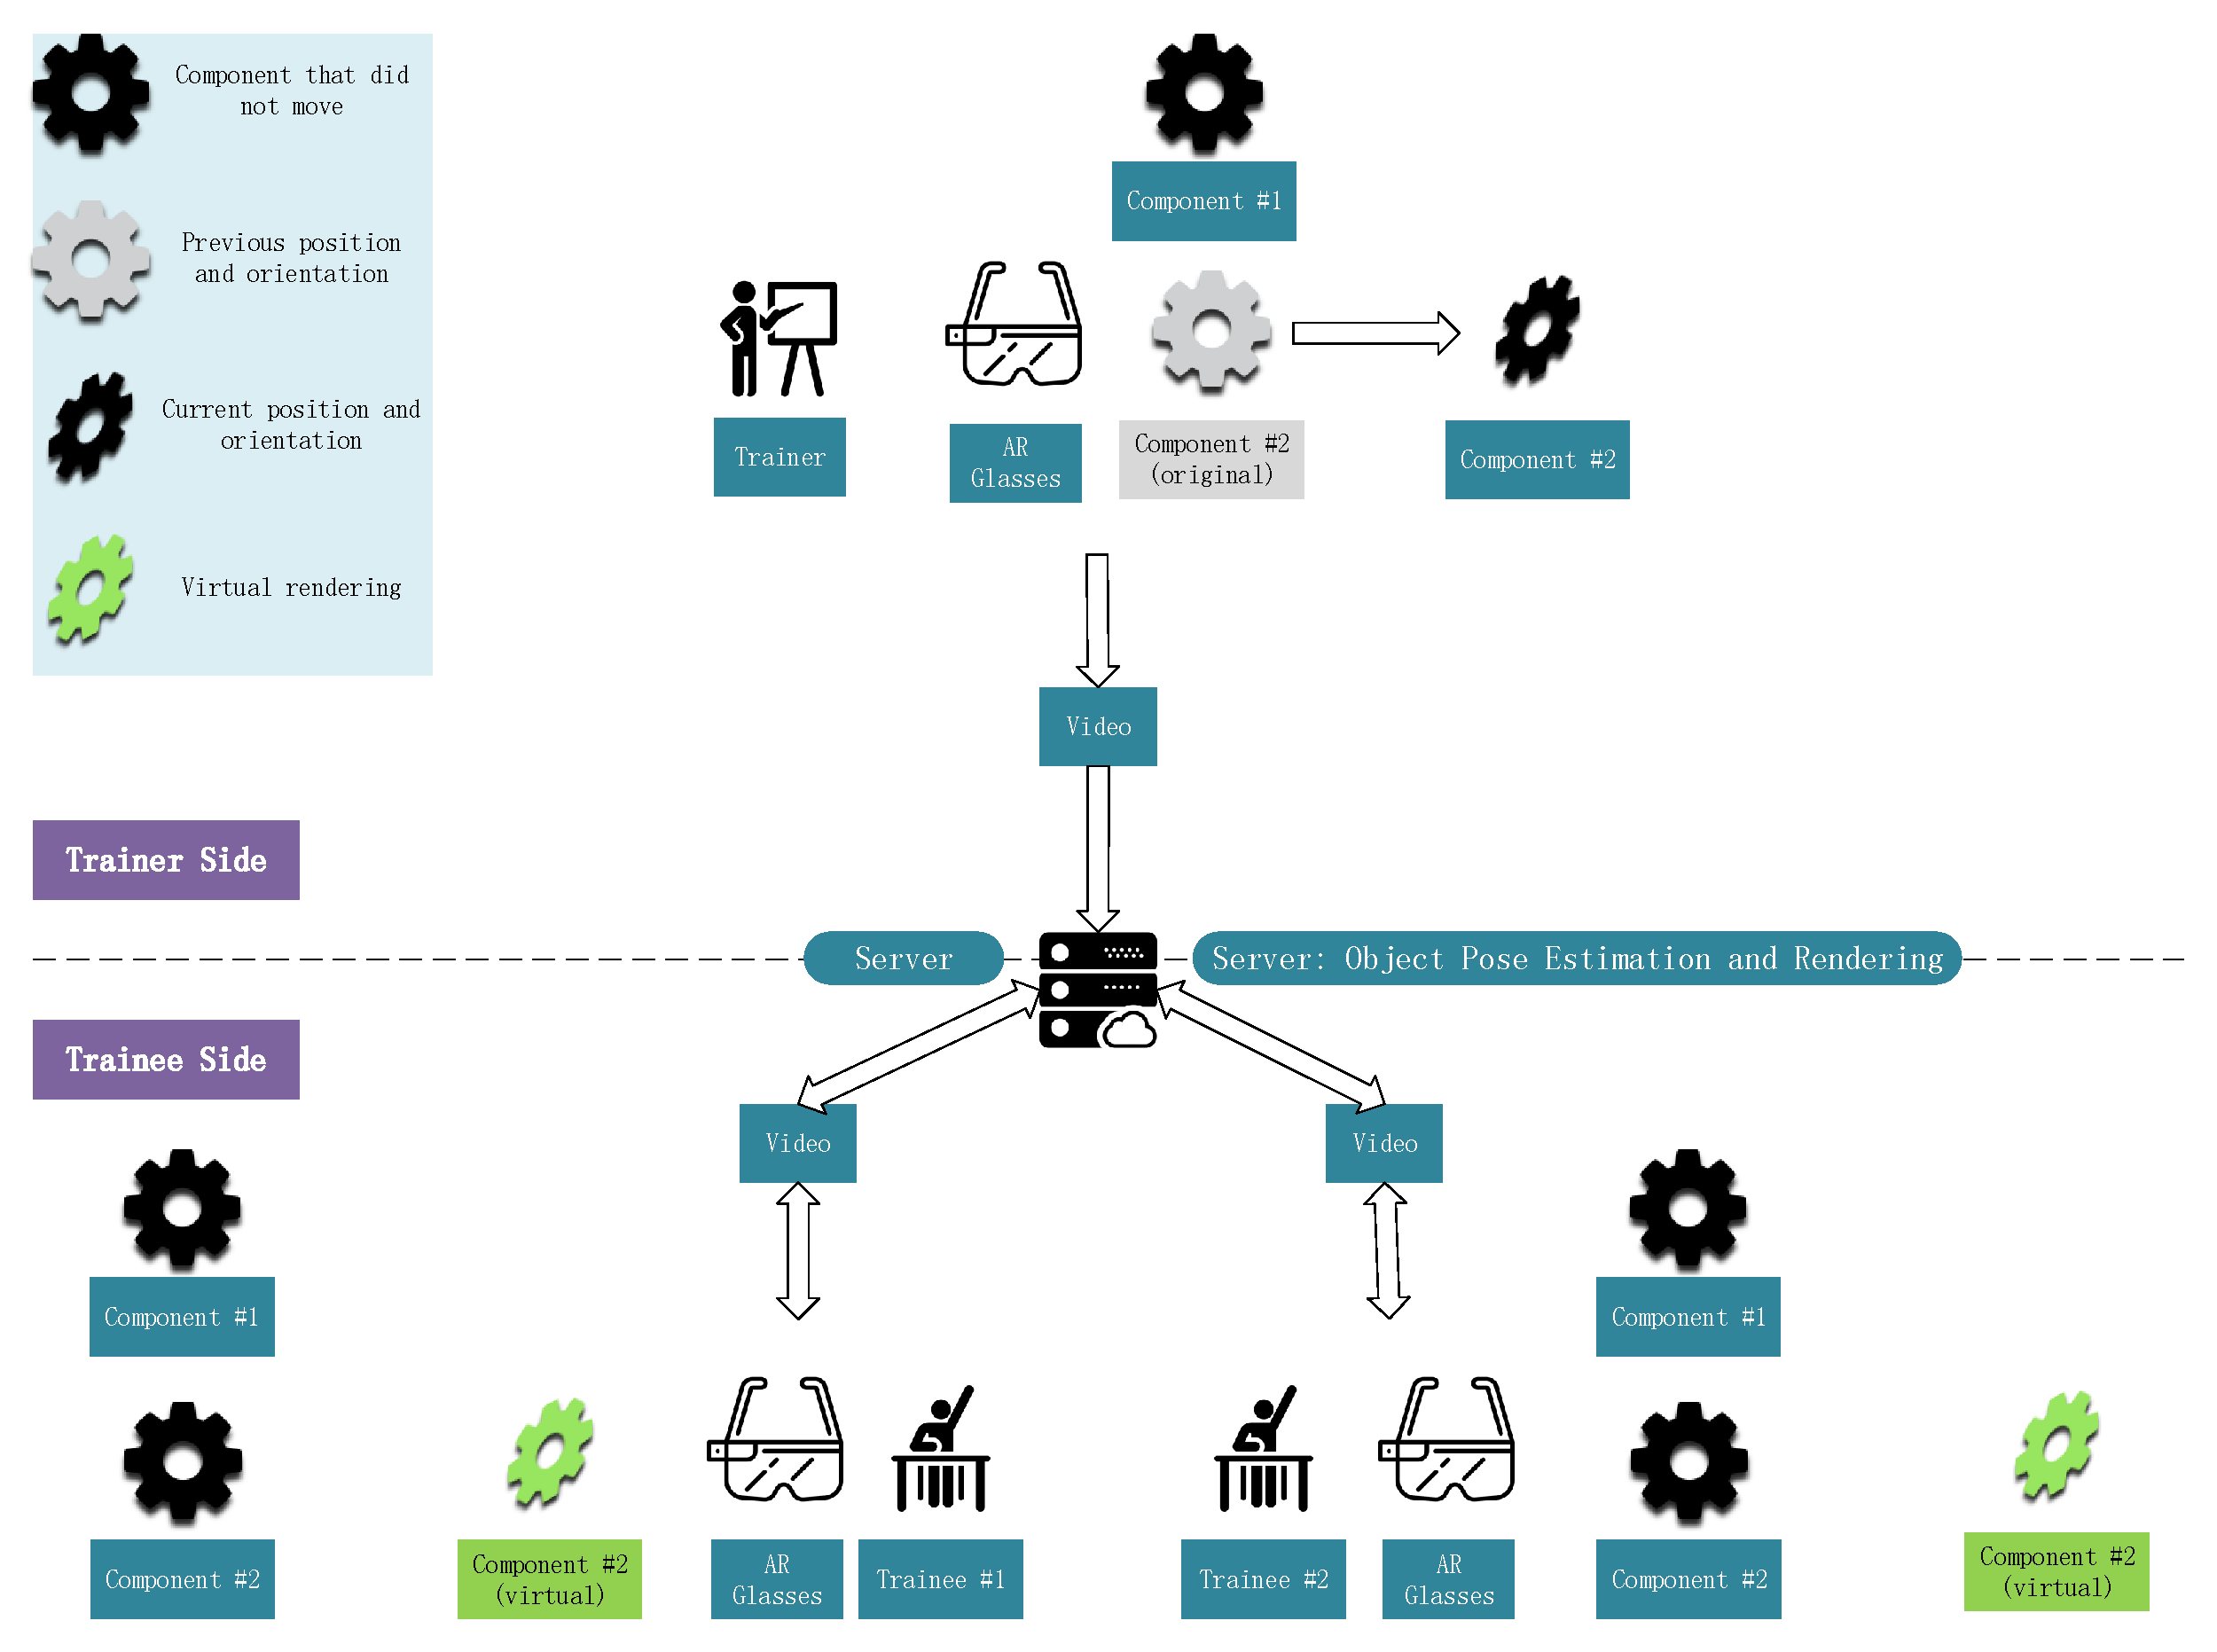
\includegraphics[width=\textwidth]{figures/scenario1.pdf}
	\caption{Training Scenario Part 1. This figure shows how the operations made by the trainer are rendered on the trainee side. The gears represent the components in the training scenario. The black gears denote the real components, while grey ones are their previous poses and the green gears demonstrate the virtual component rendered by the augmented reality devices. Moreover, the oblique gears represent the current pose after a translation and a rotation.}
	\label{fig-scenario1}
\end{figure*}

\begin{figure*}
	\centering
	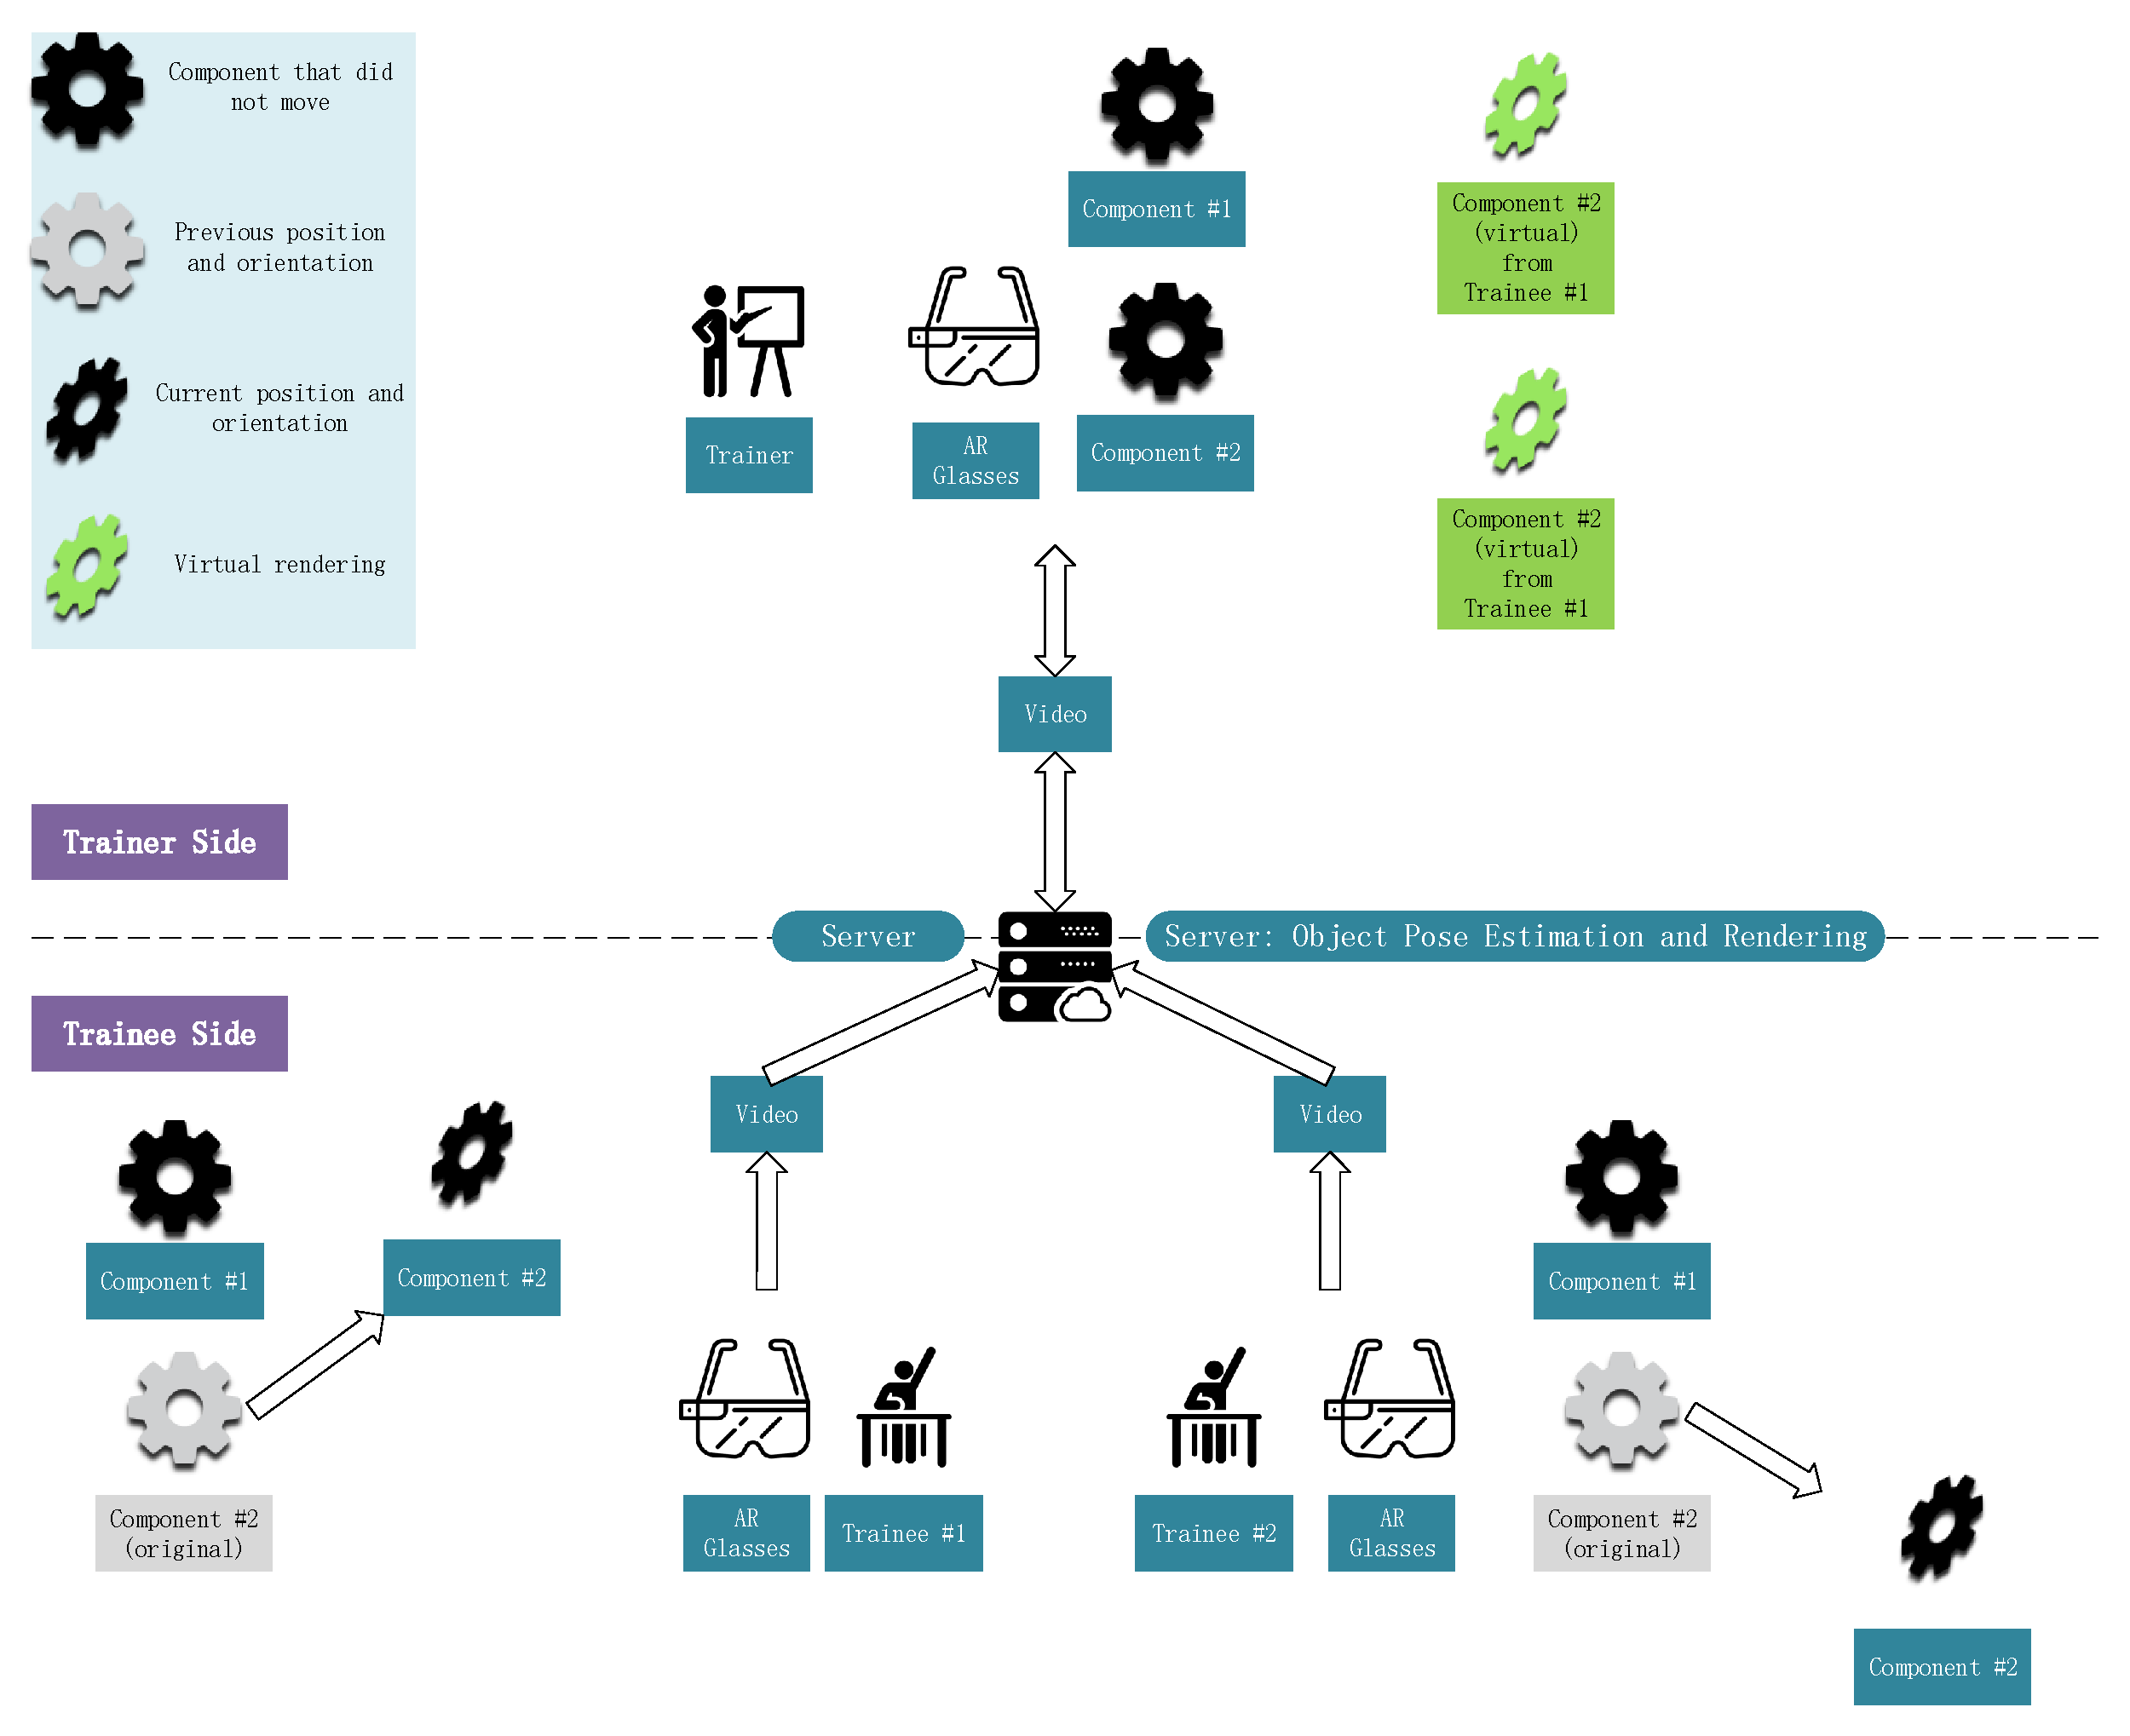
\includegraphics[width=\textwidth]{figures/scenario2.pdf}
	\caption{Training Scenario Part 2. This figure shows how the operations made by the trainees are rendered on the trainer side. The gears represent the components in the training scenario. The black gears denote the real component, while grey ones are their previous poses and the green gears demonstrate the virtual component rendered by the augmented reality devices. The oblique gears represent the current pose after a translation and a rotation.}
	\label{fig-scenario2}
\end{figure*}

Fig.~\ref{fig-scenario1} shows one of the two parts of the scenario described above. This part depicts how the trainer gives instructions to the trainees.
The upper part shows the setup of the trainer side. The grey gear represents the original pose of the component  \#2, while the black and oblique gear shows the pose of it after some operations.
The trainer wears augmented reality glasses that are equipped with a camera. The camera is used to capture videos and send them to the server.
The server estimates the pose of each component in every video frame it receives, with the CAD of all components known beforehand.
If the AR glasses is not available, a mobile device with a camera also works, e.g. a mobile phone or a tablet.

The lower part of Fig.~\ref{fig-scenario2} shows the setup of the trainee side.
There are same components in the training environment of each trainee as on the trainer side.
The trainees also wear augmented reality glasses.
Similar to the trainer side, the glasses are equipped with a camera that records videos and sends them to the server. With the video received from the trainee side, the server is able to calculate the pose of components related to each trainee.
As mentioned above, the server also estimates how the trainer moved every component on his or her side. Then it renders the 3D model of each component that has been moved, according to each trainee's view and sends it to the trainees' glasses as videos.
The black gears represent the real components on the trainee side, while the green gears show the changes made by trainer.

Fig.~\ref{fig-scenario2} demonstrates the second part of the scenario. It shows how the trainer sees the operations made by the trainees.
After receiving instructions from the trainer, each trainee perform their own operations. The operations are recorded by the camera on the augmented reality glasses as a video.
Similar to the trainer side of the first part, the server estimates how each component is moving. The estimations are performed for each video from the trainees.
Moreover, the server also receives a live video from the trainer, and calculates the pose of every component on the trainer side.
Then the server renders the components according to the operations made by each trainee, sends the virtual components to the trainer and displays them with the augmented reality glasses.
Note that a trainee may behave differently from each other, so several versions of each component are sent to the trainer. As shown in Fig.~\ref{fig-scenario2}, trainee \#1 moves component \#2 up, while trainee \#2 moves component \#2 down. Thus there are two versions of the virtual component shown in the trainer's view (marked green).

The components on the trainer side and the trainee side must be the same components, otherwise the training makes no sense. However, they do not need to be at the same location or orientation, since the server is responsible to track each component on each side.

\section{Communication Schema Design}

As shown as Fig.~\ref{fig-comm-schem}, the system consists of four services: control service, pose estimation service, rendering service and the encoding service.
The control service is responsible for controlling the entire process.
First of all, it sends requests to the pose estimation service to perform pose estimation for each client, including the trainer and all the trainees.
Note that the pose estimation service is a non-blocking service. It receives the video captured from each client independently and updates it estimation result right after receiving every frame from every client. In this way, it maintains a database of the relative pose of each object for each client. Every time it receives the request from the control service, it sends the current database to the control service.

Once the control service gets the result from the pose estimation service, it sends the pose estimation result and the rendering request to the rendering service.
When the rendering service finish rendering the models of interest for all the clients according to their point of view, it sends back the rendering result to the control service.
Note that the models of interest include the models of the components whose state (i.e. position and orientation) has been changed by the trainer but not changed accordingly by the trainees. In another word, it means the components which the trainer and the trainees need to pay attention to.

Last, the control service sends the rendering result and encoding request to the encoding service. Once the encoding service has accomplished encoding, it sends the encoded frames to each client.
The encoding service is a non-blocking service. The control service does not need to wait for the response from it to continue the process.

\begin{figure*}[!htbp]
	\centering
	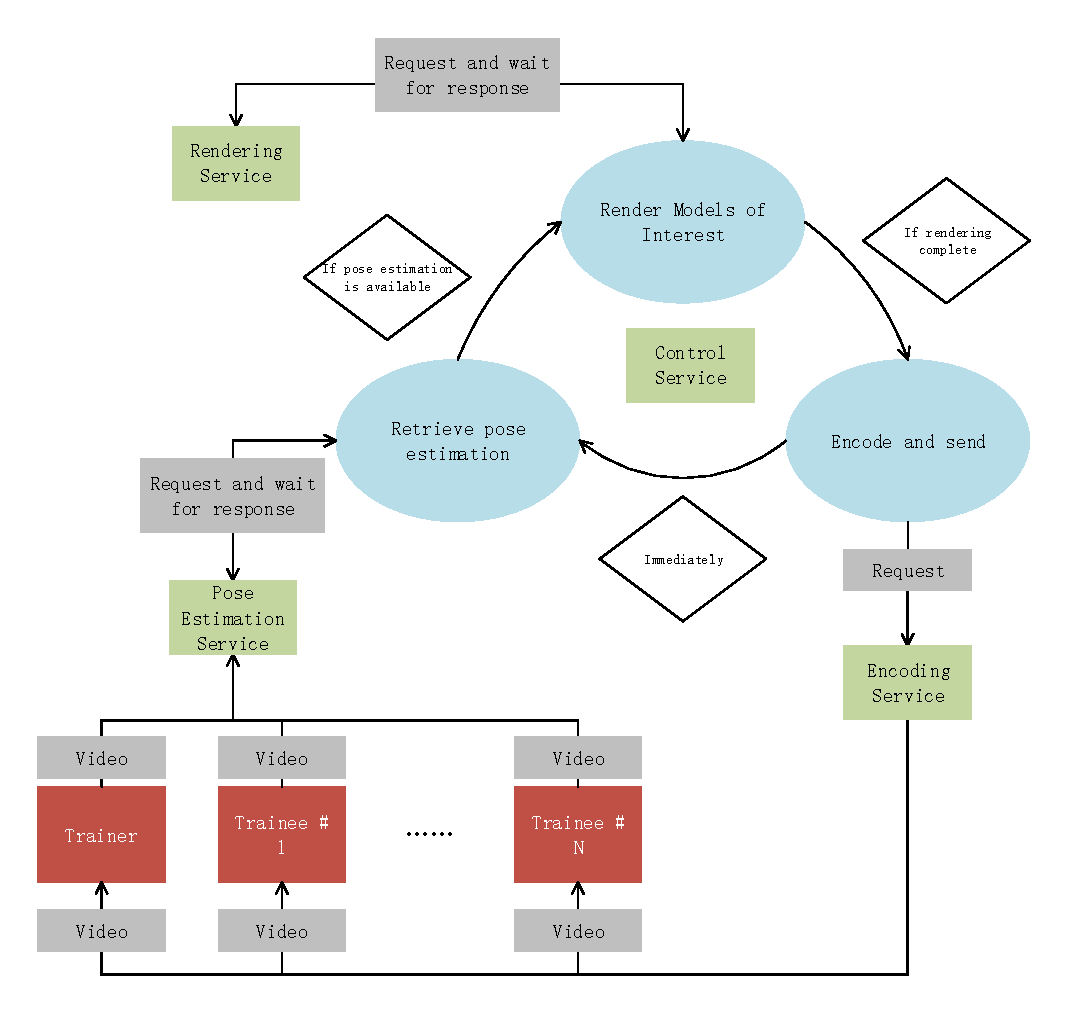
\includegraphics[width=\textwidth]{figures/communication_schema.pdf}
	\caption{Communication Schema}
	\label{fig-comm-schem}
\end{figure*}

As mentioned in Chap.~\ref{chap:hrr}, our remote rendering method includes two types of models: high-fidelity models and low-fidelity models, where the high-fidelity models are stored on the server side and the low-fidelity models are stored on the client side. Thus even without the rendering service, the clients are able to render the models if they have the basic rendering capacity.
In our schema, the only blocking service is the rendering service. For real-time performance, we set a time limit of $1/30$ second for the rendering service. If it does not accomplish the rendering within the time limit, the control service will send the pose estimation result to the clients and let them do the rendering themselves.

\section{Pose Estimation of Multiple Objects}

The first step towards our proposed framework is to estimate the poses of the objects of interest, namely the position and orientation of each object over time.
We use a model-based algorithm to estimate the poses.
With model-based pose estimation algorithms, the 3D structure of the objects of interest must be known beforehand. It is often the case in industrial training~\cite{cremers2007}.

% words need change
Some model-based approaches use edge or point features associated with the 3D models for estimating the pose~\cite{harris1990,vacchetti2004,park2008,kim2010}.
However, there are two major disadvantages with feature-based methods.
First, they struggle with motion blur and are prone to local minima especially with cluttered backgrounds.
Second, using point-based features also requires the objects' surfaces to be sufficiently textured, which significantly limits the variety of suitable objects.

% words need change
Recently, region-based pose estimation methods have emerged, which are mainly based on statistical level-set segmentation approaches.
The main advantage is that they do not require sufficiently textured objects and only reply on structure of the objects.
However, this category of approaches only work in application scenarios where it is undesirable or even impossible to modify the objects. In another word, they require the objects to be rigid. It is often the case in industrial or manufacturing training.

% words need change
In~\cite{prisacariu2012} the authors present PWP3D, the first region-based  approach that achieves real-time frame rates (20-25 Hz) using GPUs by solving the pose estimation similar to the variational approach suggested in~\cite{dambreville2010} but using level-set functions instead of separately integrating over the foreground and background region to simplify computations and make it real-time capable.
Recently, another improved PWP3D version was proposed, which runs at 30 Hz on a mobile phone~\cite{prisacariu2015}.
Tjaden et al. built an algorithm based on PWP3D, which improves convergence properties, especially for rotational motion~\cite{tjaden2016}. Also, the described implementation that uses the GPU only for rendering purposes, performs the rest computations on the CPU to achieve frame rates of about 50-100 Hz when tracking a single object on a commodity laptop.

Our method uses the work proposed by Tjaden et al.~\cite{tjaden2016} in our pose estimation service, where the object segmentation and pose estimation are performed in an interleaved fashion for each camera image.
However, the approach uses a level-set segmentation method and requires manual initialization of the segmentation, which limits its usage in real applications.
We proposed an automatic video object segmentation method, as described in Chap.~\ref{chap:vos}. In our work, the object segmentations are initialized automatically and it works with multiple objects.
Compared with other state-of-the-art automatic video object segmentation methods, our approach has the advantage that it runs in real-time.
Moreover, the synthetic silhouette that is generated with the models can be used as a ground truth segmentation, which will be used to improve the foreground and background segmentation results.

\section{Limitations}

However, the proposed framework still has several limitations.
First, the 3D models of objects involved in the training must be known beforehand, since the techniques we use in pose estimation is a model-based method.
The reason why we use a model-based pose estimation method is that this kind of methods are typically more accurate than those approaches that estimate the 3D structure and pose at the same time. Another advantage of using a model-base pose estimation method is that it does not require the presence of markers.
However, our proposed framework aims at manufacturing or assembly scenarios, in which the CAD models are typically known beforehand.
In some other training scenarios, extra effort is needed to obtain the 3D structures of the objects involved.
Second, the proposed framework does not work with non-rigid bodies.
For instance, in surgery training, the organs are deformable, it is not enough to only track the translation and orientation of an organ.
